% !TEX encoding = UTF-8
% !TEX TS-program = pdflatex
% !TEX root = ../tesi.tex
% !TEX spellcheck = it-IT

%*************************************************************
\chapter{Il contesto aziendale}
\label{cap:contesto-aziendale}
%*************************************************************

\section{L'azienda}

\myCompany è una startup avviata di recente dai due soci Marco Serpilli e David Bramini, con sede a Padova.

L'azienda è nata come spin-off di Visionest S.r.l, una società che si occupa di consulenza informatica e dello sviluppo di software gestionali dedicate alla aziende.

A differenza di Visionest, \myCompany si focalizza sulle aziende che operano nel mercato della moda e del lusso, offrendo un sistema per la gestione delle risorse e dei processi aziendali, ottimizzato per le aziende del settore.

\begin{figure}[htp]
\centering
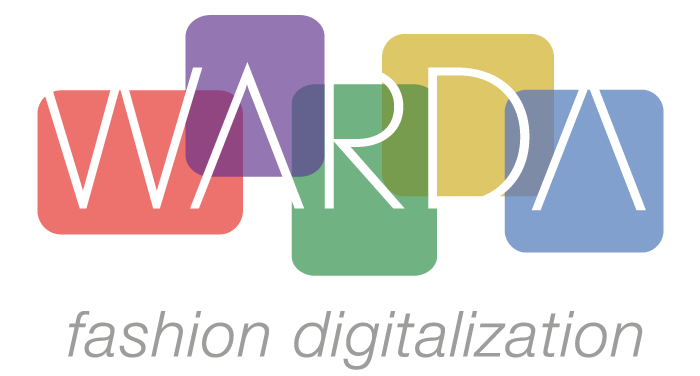
\includegraphics[width=\textwidth/2]{../immagini/warda-logo}
\caption{Logo di WARDA S.r.l.}  
\end{figure}

\subsection{WARDA - Work on what you see}

WARDA è un sistema software che si occupa di Digital Asset Management (DAM), cioè un sistema di gestione di dati digitali e informazioni di business, progettato per il mercato del lusso, fashion e retail. 

In un sistema DAM, le immagini, i video ed i documenti sono sempre legati alle informazioni di prodotto, costituendo così i digital assets: un'immagine prodotto riporta le caratteristiche della scheda prodotto, un'immagine marketing le informazioni della campagna, un'immagine della vetrina i dati del negozio, del tema, dell'ambiente, e così via.

Memorizzando questi digital assets in un unico sistema centralizzato, WARDA permette di riutilizzare infinite volte le immagini, i video e i documenti durante le attività aziendali evitando così ogni duplicazione. 

Il materiale digitale è sempre associato alla scheda prodotto gestita nel sistema informativo aziendale, rappresentando così l'unico ``catalogo digitale'' di tutti i beni/prodotti aziendali.

In questo modo WARDA diventa il centro dell'ecosistema digitale aziendale, coordinando e organizzato la raccolta e la condivisione dei digital assets attraverso processi ben definiti e istanziati secondo le prassi aziendali.

WARDA è disponibile sia come applicazione Web, sia come applicazione per iPad.

\section{Il progetto}
Lo scopo del progetto è quello di valutare se, mediante l'utilizzo di framework differenti, sia possibile migliorare l'esperienza d'uso del client per iPad di WARDA.

Secondo l'azienda la causa di alcuni problemi del client attuale derivano dal framework che è stato utilizzato per svilupparlo, infatti, l'applicazione attuale è un'applicazione di tipo ibrido, cioè composta da un'applicazione web ottimizzata per lo schermo dell'iPad e racchiusa in un'applicazione nativa utilizzando Cordova.

Di conseguenza, si ritiene che l'utilizzo di un'altra tipologia di framework che permette lo sviluppo di applicazioni native utilizzando JavaScript possa portare dei miglioramenti all'applicazione attuale.

Pertanto, la prima parte del progetto riguarda la ricerca e l'analisi di framework che permettono di sviluppare applicazioni native con JavaScript utilizzando un'interfaccia grafica nativa al posto di una pagina web.

La seconda parte invece, prevede lo sviluppo di un'applicazione analoga a al client per iPad attuale utilizzando uno dei framework individuati.
